\documentclass[]{beamer}
\usetheme{CambridgeUS}

%%%%%
% typesetting
%%%%%
\usepackage[OT1]{fontenc}   % 
\usepackage[utf8]{inputenc} % enables use of æ,ø,å
\usepackage[danish,german,english]{babel}
\usepackage{lmodern}


%%%
% verbatim
%%%
\usepackage{verbatim}
\usepackage{fancyvrb} % for \Verb + \Verbatiminput

%%%%
% general packages
%%%%
%\usepackage{etex} % extended tex, for using more than 256 registers for coding

% make danish text with æøå
\newcommand{\textdanish}[1]%
{%
      \foreignlanguage{danish}{#1}%
}

%%%%
% code listing
%%%%
\usepackage{xcolor}
\usepackage{listings}

%%%%
% math
%%%%
\usepackage{amsmath}
\usepackage{amsfonts}
\usepackage{amssymb}

%%%%
% tikz/graphics
%%%%
\usepackage{tikz}
%\usetikzlibrary{arrows.meta}
\usetikzlibrary{arrows}
\usetikzlibrary{calc}
\usetikzlibrary{decorations.pathreplacing}
\usetikzlibrary{decorations.markings}
\usepackage{graphicx}
\usepackage{subcaption} % for subfigure

%%%%%
% for tabulars
%%%%%
\usepackage{multirow}

%%%%
% text colorbox
%%%%
\usepackage[listings,most]{tcolorbox}
\tcbset{
  colback=black,
}

\newcommand{\hiddenhint}[1] %
{ %
\newline
\begin{tcolorbox}{ {\color{black} \emph{Hint:} } {#1} } \end{tcolorbox}
%\begin{tcolorbox}{\color{black} \emph{Hint:} } {#1}\end{tcolorbox}
%\emph{HiddenHint:} {#1}
} %

\newcommand{\hint}[1] %
{ %
\emph{Hint:} {#1}
} %

%%%%%
% spaces
%%%%%
\newcommand{\verticalspace}{\vspace{0.3cm}}
\newcommand{\mediumverticalspace}{\vspace{0.2cm}}
\newcommand{\smallverticalspace}{\vspace{0.1cm}}
\newcommand{\horizontalspace}{\hspace{1cm}}

%%%%
%
% includes needed
%
%%%%
\usepackage{color}
\usepackage{xcolor}
\usepackage[margin=10pt]{caption}
\usepackage{listings}
\usepackage{fancyvrb} % for \Verb

%%%%
%
% General settings
%
%%%%
% color setup
\definecolor{listinggray}{gray}{0.98}
%\colorlet{listinggray}{gray!40}
\definecolor{lbcolor}{rgb}{0.9,0.9,0.9}

\lstset{
   frame=tb
 , frameround=ftft
 , numbers=left      % put code line numbers on left
 , numberstyle=\tiny\color[rgb]{0.205, 0.142, 0.73}% size of line numbers
 , numbersep=5pt
 , xleftmargin=\parindent % set left margin to paragraph indention
 , captionpos=tl
 %, backgroundcolor=\color{lbcolor}
 , backgroundcolor=\color{listinggray}
 , keywordstyle=\color[rgb]{0,0,1}
 , commentstyle=\color{violet}
 , stringstyle=\color{red}
 , basicstyle=\ttfamily\lst@ifdisplaystyle\scriptsize\fi
}

% set code size
%\def{\codesize}{\lst@ifdisplaystyle\scriptsize\fi}

\newcommand{\inlinecode}[2][cpp]{\lstinline[style=custom#1,prebreak=]{#2}}
\newcommand{\includecode}[3][cpp]{\lstinputlisting[caption={#2 \hfill
\texttt{\scriptsize (\lstname)}},style=custom#1]{#3}}

% caption setup
\DeclareCaptionLabelFormat{advancedlabelformat}{[ #1 ]}
%\DeclareCaptionFormat{advancedformat}{\colorbox{cmyk}{0.43, 0.35, 0.35,0.01}{\parbox{\textwidth}{#1 #3}}}
\DeclareCaptionFormat{advancedformat}{#1 #3}
\captionsetup[lstlisting]{
   format=advancedformat
 , labelformat=advancedlabelformat
}


%%%%
%
% Cpp enviroment
%
%%%%
\newcommand{\cppname}{{C{}\Verb|++|}} % name of cpp listings

% cpp style
\lstdefinestyle{customcpp}{
   language=[ISO]C++
 %, keywordstyle=\color{red!20!darkgreen}\bfseries
 %, keywordstyle=\color{yellow!60!green}\bf
 %, commentstyle=\color{blue}
 %, stringstyle=\ttfamily\color{red!50!brown}
 , showstringspaces=false
 , escapechar=£
 %, basicstyle=\ttfamily\codesize
 , flexiblecolumns=true
 , keywords=[2]{final,override,nullptr,uchar,size_t}
 %, literate=%
 %     *{0}{{{\color{red!20!violet}0}}}1
 %      {1}{{{\color{red!20!violet}1}}}1
 %      {2}{{{\color{red!20!violet}2}}}1
 %      {3}{{{\color{red!20!violet}3}}}1
 %      {4}{{{\color{red!20!violet}4}}}1
 %      {5}{{{\color{red!20!violet}5}}}1
 %      {6}{{{\color{red!20!violet}6}}}1
 %      {7}{{{\color{red!20!violet}7}}}1
 %      {8}{{{\color{red!20!violet}8}}}1
 %      {9}{{{\color{red!20!violet}9}}}1
}

% cpp environment
\lstnewenvironment{cpp}[1][]
{ 
   \renewcommand\lstlistingname{\cppname{}}
   \lstset{style=customcpp,caption={#1 \hfill \ }}
}
{ }

% inline cpp
\newcommand{\icpp}[1]{
   \inlinecode[cpp]{#1}
}

% include cpp file
\newcommand{\includecpp}[2][]{
   \renewcommand\lstlistingname{\cppname{}}
   \includecode[cpp]{#1}{#2}
}


%%%%
%
% Fortran
%
%%%%
\newcommand{\fortranname}{FORTRAN}

\lstdefinestyle{customfortran}{
   language=fortran
 , basicstyle=\ttfamily\codesize
}

\lstnewenvironment{fortran}[1]
{ 
   \renewcomman\lstlistingname{\fortranname{}}
   \lstset{style=customfortran,caption={#1 \hfill \ }} 
}
{ }

\newcommand{\ifortran}[1]{\inlinecode[fortran]{#1}}



%%%%%
%
% Assembly
%
%%%%%
\newcommand{\asmname}{ASM}

\lstdefinestyle{customasm}{
   language=[x86masm]Assembler
 %, basicstyle=\codesize\ttfamily
 , commentstyle=\itshape\color{purple!40!black}
}

\lstnewenvironment{asm}[1]
{
   \renewcommand\lstlistingname{\asmname{}}
   \lstset{style=customasm,caption={#1 \hfill \ }} 
}
{ }

\newcommand{\iasm}[1]{\inlinecode[asm]{#1}}

%%%%
% bash
%%%%
\newcommand{\bashname}{Bash}

\lstdefinestyle{custombash}{
   language=bash
 %, basicstyle=\codesize\ttfamily
}

\lstnewenvironment{bash}[1]
{
   \renewcommand\lstlistingname{\bashname{}}
   \lstset{style=custombash,caption={#1 \hfill \ }} 
}
{ }

\newcommand{\includebash}[2][]{
   \renewcommand\lstlistingname{\bashname{}}
   \includecode[bash]{#1}{#2}
}

%%%%
% terminal
%%%%%
\lstdefinestyle{customterminal}{
   language=bash
 %, backgroundcolor=\color{white}
 , backgroundcolor=\color{listinggray}
 , keywordstyle=\color{black}
 , commentstyle=\color{black}
 , stringstyle=\color{black}
 , numberstyle=\color{black}
 , frame=
 , numbers=none  % put code line numbers on left
 %, basicstyle=\codesize\ttfamily
}

%\newenvcommand{terminal}{\command}[1]
%{
%$ #1
%}

\lstnewenvironment{terminal}[1][]
{
 % \checkenvcommand
  \renewcommand\lstlistingname{Terminal}
  \lstset{style=customterminal,caption={#1 \hfill \ }} 
}
{ }

\newcommand{\iterminal}[1]{\inlinecode[terminal]{#1}}

%%%%
%
% ls.tex
%
%%%%

\usepackage{fancyvrb}

\def\lscounter{0}
\newcommand{\lsoutput}{}
\newcommand{\lscommand}{}

\newcommand{\ifsecondboth}[2]{
  \if #2\empty
    \empty
  \else
    #1#2
  \fi
}

\newcommand{\ls}[2][]{
  \renewcommand{\lsoutput}{lsoutput\lscounter.tex}
  \renewcommand{\lscommand}{ls \ifsecondboth{-}{#1} #2}
  \immediate\write18{\lscommand > \lsoutput}
  %\Verb{test}
  {\scriptsize \texttt{\$ \lscommand} }
  \VerbatimInput[fontsize=\scriptsize]{\lsoutput}
  \count0=\lscounter\relax % put lscounter in to register 0
  \advance\count0 by 1     % advance counter by 1
  \def\lscounter{\the\count0} % put counter back into lscounter
}


\usepackage{tikzsymbols}

% nice looking math
\usefonttheme[onlymath]{serif}

% Define some colors 
\definecolor{cambridge}{RGB}{163,00,00}
\definecolor{ultramarine}{RGB}{0,32,96}

% Nice looking blocks
\setbeamercolor{block title}{bg=cambridge,fg=white}
\setbeamercolor{block body}{bg=cambridge!20,fg=black}

% Nice itemize
\setbeamercolor{itemize item}{fg=cambridge}
\setbeamercolor{itemize subitem}{fg=ultramarine}
\setbeamercolor{itemize subsubitem}{fg=cyan}

\setbeamertemplate{itemize item}[square]
\setbeamertemplate{itemize subitem}[triangle]
\setbeamertemplate{itemize subsubitem}[circle]

% Nice enumerate
\setbeamertemplate{enumerate item}[square]
\setbeamertemplate{enumerate subitem}[triangle]
\setbeamertemplate{enumerate subsubitem}[circle]
\setbeamercolor{enumerate item}{fg=cambridge}
\setbeamercolor{enumerate subitem}{fg=ultramarine}
\setbeamercolor{enumerate subsubitem}{fg=cyan}
\setbeamercolor{local structure}{fg=cambridge}

\begin{document}
\title{Neural Networks}

%%%%%%%%%%%%%%%%%%%%%%%%%%%%%%%%%%%%%%%%%%%%%%%%
% Intro
%%%%%%%%%%%%%%%%%%%%%%%%%%%%%%%%%%%%%%%%%%%%%%%%
\begin{frame}
\titlepage
\end{frame}

\begin{frame}
   {Inspiration}
   \begin{figure}
      \centering
      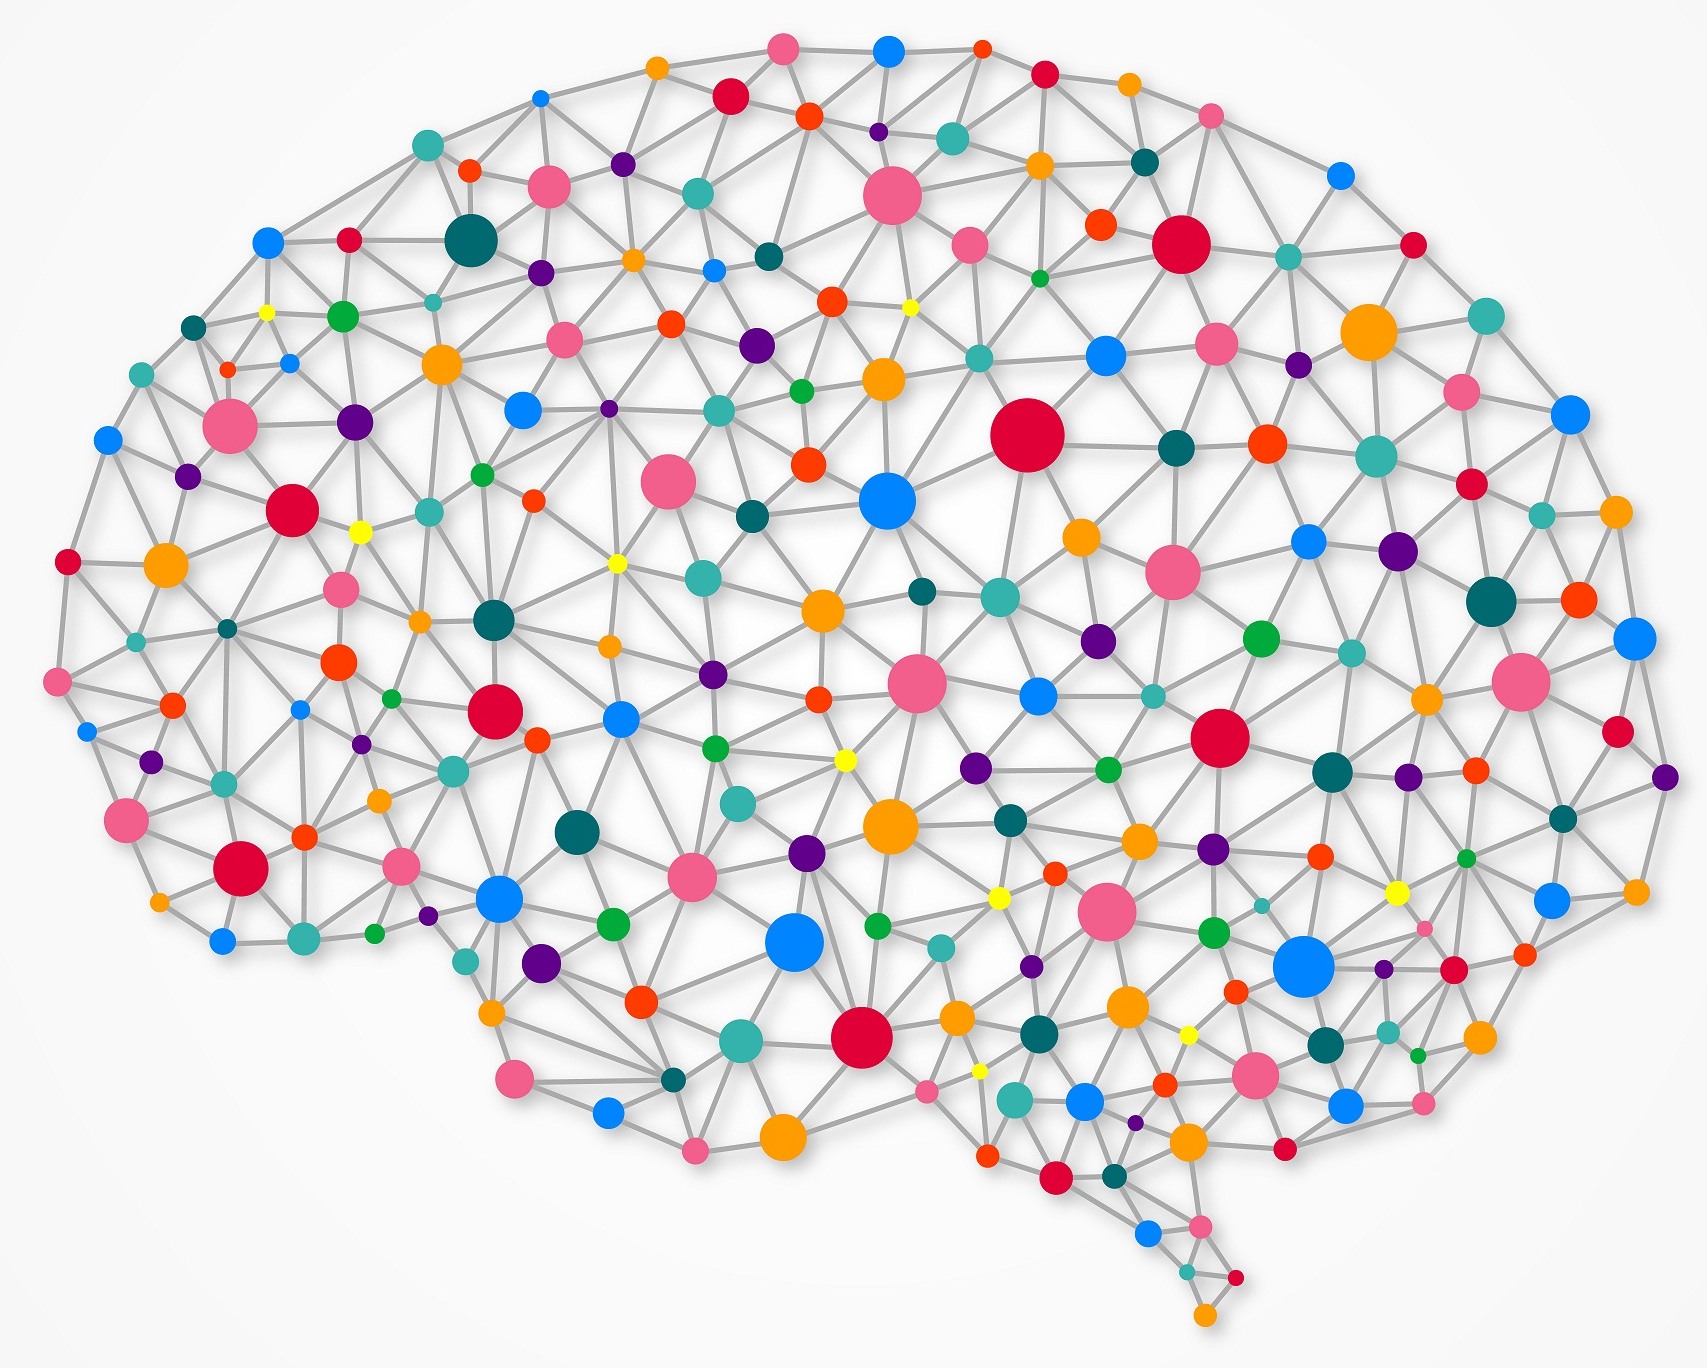
\includegraphics[width=0.75\linewidth]{figures/brain_network_crop.jpg}
   \end{figure}
\end{frame}

%%%%%%%%%%%%%%%%%%%%%%%%%%%%%%%%%%%%%%%%%%%%%%%%
% 
%%%%%%%%%%%%%%%%%%%%%%%%%%%%%%%%%%%%%%%%%%%%%%%%
\begin{frame}[fragile]
   {Feed-forward Artificial Neural Network (ANN)}
   \begin{figure}
      \centering
      \includegraphics[scale=1.1]{figures/neural_network/neural_network-figure0.pdf}
   \end{figure}
\end{frame}

% Xor-gate
\begin{frame}
   {Motivating example: XOR (Exclusive Or)}
   \scriptsize
   \vspace{-0.2cm}
   \begin{minipage}{0.32\linewidth}
      \centering
      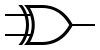
\includegraphics[width=0.7\linewidth]{figures/xor_gate.png}
   \end{minipage}
   \begin{minipage}{0.32\linewidth}
      \centering
      \begin{equation*}
         \mathcal{O} = \left(A + B \right) \cdot \overline{\left( A \cdot B \right)}
      \end{equation*}
   \end{minipage}
   \begin{minipage}{0.32\linewidth}
      \centering
      \begin{equation*}
         \begin{array}{ccc}
            A & B & \mathcal{O} \\ \hline
            0 & 0 & 0 \\
            0 & 1 & 1 \\
            1 & 0 & 1 \\
            1 & 1 & 0 \\
         \end{array}
      \end{equation*}
   \end{minipage}
   \vspace{0.2cm}
   Choosing a linear model:
   \begin{equation*}
      f \left(\boldsymbol{x}; \boldsymbol{w}, b \right) = \boldsymbol{x}^T \boldsymbol{w} + b
   \end{equation*}
   we get $\boldsymbol{w} = \boldsymbol{0}$ and $b = \frac{1}{2}$, \emph{i.e.} the linear model outputs $0.5$ everywhere.
   
   \vspace{0.2cm}
   \begin{figure}
      \centering
      \includegraphics[width=0.275\linewidth]{figures/xor_plot/xor_plot-figure0.pdf}
      %\hspace{2cm}
      %\includegraphics[width=0.275\linewidth]{figures/xor_plot/xor_plot-figure1.pdf}
   \end{figure}
\end{frame}

\begin{frame}
   {Learning with simple Feedforward Network}
   \scriptsize
   \begin{minipage}{0.475\linewidth}
      \begin{itemize}
         \item
            One hidden layer with two units.
         \item
            Two step process: 
            \begin{itemize}
               \item
                  $\boldsymbol{h} = f^{(1)} \left( \boldsymbol{x}; \boldsymbol{W}, \boldsymbol{c} \right)$
               \item
                  $y = f^{(2)} \left( \boldsymbol{h}; \boldsymbol{w}, b \right)$
            \end{itemize}
         \item
            The complete model looks like:
            \begin{equation*}
            %\begin{itemize}
            %   \item
                  f \left(\boldsymbol{x}; \boldsymbol{W}, \boldsymbol{c}, \boldsymbol{w}, b \right) = f^{(2)}\left(f^{(1)}\left( \boldsymbol{x} \right) \right)
            %\end{itemize}
            \end{equation*}
         \item
            What should $f^{(1)}$ and $f^{(2)}$ look like?
      \end{itemize}

   \end{minipage}
   \begin{minipage}{0.475\linewidth}
      \begin{figure}
         \includegraphics[width=\linewidth]{figures/xor/xor-figure0.pdf}
      \end{figure}
   \end{minipage}
   
   \vspace{1cm}
   Choosing both $f^{(1)}$ and $f^{(2)}$ as linear models we end up with a linear model.
   \begin{equation*}
      f^{(1)} = \boldsymbol{W}^T \boldsymbol{x}, \quad f^{(2)} = \boldsymbol{h}^T \boldsymbol{w} \quad \implies \quad f(\boldsymbol{x}) = \boldsymbol{w}^T \boldsymbol{W}^T \boldsymbol{x}
   \end{equation*}
   Clearly we need one of the functions to be non-linear!
\end{frame}

\begin{frame}
   {Rectified Linear Unit (ReLU)}
   \scriptsize
   \begin{minipage}{0.475\linewidth}
      \begin{itemize}
         \item
            We want to chose $f^{(1)}$ as a non-linear function.
         \item
            Modern neural networks employs Rectified linear units.
            \begin{equation*}
               g(z) = \max(0, z)
            \end{equation*}
         \item
            We then get:
            \begin{equation*}
               f^{(1)} = \max(0, \boldsymbol{W}^T \boldsymbol{x} + \boldsymbol{c})
            \end{equation*}
      \end{itemize}
   \end{minipage}
   \begin{minipage}{0.475\linewidth}
   \begin{figure}
      \includegraphics[scale=0.5]{figures/activation_functions/activation_function-figure0.pdf}
   \end{figure}
   \end{minipage}
   
   \vspace{1cm}

   Our complete model becomes:
   \begin{equation*}
      f\left( \boldsymbol{x}; \boldsymbol{W}, \boldsymbol{c}, \boldsymbol{w}, b \right) = \boldsymbol{w}^T \max \left(0, \boldsymbol{W}^T \boldsymbol{x} + \boldsymbol{c} \right) + b
   \end{equation*}
\end{frame}

\begin{frame}
   {Non-linear}
   \begin{figure}
      \centering
      \includegraphics[width=\linewidth]{figures/xor_model/xor_model-figure0.pdf}
   \end{figure}
   \begin{figure}
      \centering
      \includegraphics[width=\linewidth]{figures/xor_model/xor_model-figure1.pdf}
   \end{figure}
\end{frame}

\begin{frame}
   {General Feedforward network}
   \scriptsize
   \begin{figure}
      \includegraphics[width=\linewidth]{figures/general_feedforward_2/general_feedforward-figure0.pdf}
   \end{figure}
   
   \begin{itemize}
      \item
         A feedforward network consist of layers of neurons.
      \item
         The output of neurons in layer $n$ is passed as input to the neurons in layer $n + 1$
   \end{itemize}
\end{frame}

% Perceptron
\begin{frame}[fragile]
   {Neuron/Perceptron}
   \scriptsize
   \begin{minipage}{0.475 \linewidth}
      \setbeamercolor{enumerate item}{fg=cambridge}
      \begin{enumerate}
         \item
            \textbf{Perceptron} recieves input $\boldsymbol{h}^{(i)} = \left( h^{(i)}_1, h^{(i)}_2, \dots, h^{(i)}_m \right)$ from previous layer.
            If a \textbf{bias} is included in the model add a fixed $h^{(i)}_0 = 1$ to the input.
         \item
            Inputs are multiplied by the \textbf{Synaptic Weights},
            and added together at the \textbf{Summing Junction} (Linear/Affine transformation).
            \begin{equation*}
               v_k = \boldsymbol{w}^T_k \boldsymbol{h}^{(i)} = \sum_{j=0}^m w_{kj} h^{(i)}_j
            \end{equation*}
         \item
            \textbf{Activation function} is evaluated to give \textbf{Perceptron} output (Non-linear transformation).
            \begin{equation*}
               h^{(o)}_k = f \left( v_k \right)
            \end{equation*}
      \end{enumerate}

   \end{minipage}
   \hspace{-0.2cm}
   \begin{minipage}{0.475 \linewidth}
      %\begin{figure}
      %   \centering
      %   \includegraphics[width=1.0\linewidth]{figures/neuron/neuron-figure0.pdf}
      %\end{figure}
      \vspace{-0,5cm}
      \begin{figure}
         \centering
         \includegraphics[width=1.15\linewidth]{figures/neuron_bias_2/neuron-figure0.pdf}
      \end{figure}
   \end{minipage}
\end{frame}

\begin{frame}
   {Feeding forward}
   \begin{minipage}{0.475\linewidth}
   \begin{figure}
      \includegraphics[width=1.1\linewidth]{figures/neural_network_detail_2/neural_network_detail-figure0.pdf}
   \end{figure}
   \end{minipage}
   \begin{minipage}{0.475\linewidth}
   \begin{figure}
      \includegraphics[width=1.1\linewidth]{figures/neural_network_detail/neural_network_detail-figure0.pdf}
   \end{figure}
   \end{minipage}
   \scriptsize
   \vspace{0.4cm}
   \begin{center}
   \begin{itemize}
      \item
         Each Perceptron in layer $n$ sends its output to each Perceptron in layer $n + 1$.
      \item
         Each Perceptron in layer $n + 1$ recieves input from all Perceptrons in layer $n$.
   \end{itemize}
   \end{center}
\end{frame}

\begin{frame}
   {Evaluating a feedforward network}
   \scriptsize
   Evaluating Perceptron $k$ in layer $n$
   \begin{equation*}
      h^{(n)}_k = f^{(n)}_k \left( \boldsymbol{w}^{(n)T}_k \boldsymbol{h}^{(n-1)} \right) 
   \end{equation*}
   Evaluating the whole network is just a question of evaluating each layer in succession, i.e. \textbf{Feed-forward}.
   \begin{equation*}
      h^{(1)}_k = f^{(1)}_k \left( \boldsymbol{w}^{(1)T}_k \boldsymbol{h}^{(0)} \right) 
   \end{equation*}
   \begin{equation*}
      h^{(2)}_k = f^{(2)}_k \left( \boldsymbol{w}^{(2)T}_k \boldsymbol{h}^{(1)} \right) 
   \end{equation*}
   \begin{equation*}
      \dots
   \end{equation*}
   \begin{equation*}
      h^{(O)}_k = f^{(O)}_k \left( \boldsymbol{w}^{(O)T}_k \boldsymbol{h}^{(O-1)} \right) 
   \end{equation*}
   
   \vspace{0.4cm}
   If all neurons in a layer has the same activation function we can rewrite the layer evaluation:
   \begin{equation*}
      \boldsymbol{h}^{(n)} = f^{(n)} \left( \boldsymbol{W}^{(n)T} \boldsymbol{h}^{(n-1)} \right)
   \end{equation*}
\end{frame}

\begin{frame}
   {Activation functions}
   \begin{figure}
      \includegraphics[width=0.30\linewidth]{figures/activation_functions/activation_function-figure0.pdf}
      \hspace{0.1cm}
      \includegraphics[width=0.30\linewidth]{figures/activation_functions/activation_function-figure1.pdf}
      \hspace{0.1cm}
      \includegraphics[width=0.30\linewidth]{figures/activation_functions/activation_function-figure2.pdf}
   \end{figure}
   \begin{figure}
      \includegraphics[width=0.30\linewidth]{figures/activation_functions/activation_function-figure3.pdf}
      \hspace{0.1cm}
      \includegraphics[width=0.30\linewidth]{figures/activation_functions/activation_function-figure4.pdf}
      \hspace{0.1cm}
      \includegraphics[width=0.30\linewidth]{figures/activation_functions/activation_function-figure5.pdf}
   \end{figure}
   %\begin{figure}
   %\end{figure}
\end{frame}


\begin{frame}
   {Minimization}
   \scriptsize
   Optimizing the weight of a feedforward neural network is a minimization problem!
   \begin{block}
      {Optimization}
      To optimize the weights of out network, we want, given a training set $\boldsymbol{x} \in \mathbb{X}$, to minimize a loss function $J \left( \boldsymbol{w} \right)$ over the training set. This could e.g. be a sum of squares loss function
      \begin{equation*}
         J \left( \boldsymbol{w} \right) = \frac{1}{2} \sum_{\boldsymbol{x} \in \mathbb{X}} \left( f^*\left(\boldsymbol{x}\right) - f \left(\boldsymbol{x}; \boldsymbol{w} \right) \right)^2
      \end{equation*}
      The equation is at an optimum if the gradient is w.r.t. the weights is $\boldsymbol{0}$
      \begin{equation*}
         \frac{\partial }{\partial \boldsymbol{w}} J \left( \boldsymbol{w} \right) 
            = \boldsymbol{0}
      \end{equation*}
   \end{block}
   
   \vspace{0.5cm}
   We thus need derivatives of the loss function with respect to all linear weights $\boldsymbol{w}_{kj}$ of the Perceptrons.
   \begin{equation*} 
      \frac{\partial J \left( \boldsymbol{w} \right)}{\partial w_{kj}} = 0
   \end{equation*}
\end{frame}

%\begin{frame}
%   {Vector differentiation}
%   \begingroup
%   \renewcommand*{\arraystretch}{1.5}
%   \begin{equation*}
%      \frac{\partial}{\partial \boldsymbol{\theta}} J \left(\boldsymbol{\theta}\right) = 
%      \begin{bmatrix}                
%         {\partial J \left( \boldsymbol{\theta} \right) \over \partial \theta_{1} } \\
%         {\partial J \left( \boldsymbol{\theta} \right) \over \partial \theta_{2} } \\
%            \vdots \\ 
%         {\partial J \left( \boldsymbol{\theta} \right) \over \partial \theta_{n} } \\
%      \end{bmatrix}
%   \end{equation*}
%   \endgroup
%\end{frame}


\begin{frame}
   {Back-propagation: Chain-rule}
   \begin{block}
      {Chain-rule}
      Let $\boldsymbol{x} \in \mathbb{R}^m$, $\boldsymbol{y} \in \mathbb{R}^n$, $g: \mathbb{R}^m \rightarrow \mathbb{R}^n$, and $f: \mathbb{R}^m \rightarrow \mathbb{R}$.
      If $\boldsymbol{y} = g \left( \boldsymbol{x} \right)$ and $z = f \left( \boldsymbol{y} \right)$, then:
      \begin{equation*}
         \frac{\partial z}{\partial x_i} = \sum_j \frac{\partial z}{\partial y_j} \frac{\partial y_j}{\partial x_i}
      \end{equation*}
      Written in vector notation we get,
      \begin{equation*}
         \nabla_{\boldsymbol{x}} z = \left( \frac{\partial \boldsymbol{y}}{\partial \boldsymbol{x}} \right)^T \nabla_{\boldsymbol{y}} z,
      \end{equation*}
      where $\frac{\partial \boldsymbol{y}}{\partial \boldsymbol{x}}$ is the $n \times m$ Jacobian of $g$.
   \end{block}

   %\begin{itemize}
   %   \item
   %      Can also be generalised to tensor of arbitrary order.
   %\end{itemize}
\end{frame}

\begin{frame}
   {Graph derivative: Example}
   \begin{figure}
      \includegraphics[width=0.7\linewidth]{figures/derivative_graph/derivative_graph-figure0.pdf}
   \end{figure}
\end{frame}

\begin{frame}
   {Backpropagation derivation}
   \scriptsize
   \begin{block}
      {Definition $\alpha^{(n)}_k$}
      Remember that the output of layer $n$ can be written as
      \begin{equation*}
         h^{(n)}_k = f^{(n)}_k \left( \boldsymbol{w}^{(n)T}_k \boldsymbol{h}^{(n-1)} \right) 
                   = f^{(n)}_k \left( \alpha^{(n)}_k \right)
      \end{equation*}
      with the definition
      \begin{equation*}
         \alpha^{(n)}_k = \boldsymbol{w}^{(n)T}_k \boldsymbol{h}^{(n-1)} = \sum_i w_{ki}^{(n)} h^{(n-1)}_i
      \end{equation*}
   \end{block}
   
   As $w^{(n)}_{ki}$ only enters the loss function through $\alpha^{(n)}_k$ we can, using the Chain rule, write the gradient of the loss function as:
   \begin{equation*}
      \frac{\partial J\left(\boldsymbol{w} \right)}{\partial w_{ki}^{(n)}} = \frac{\partial J \left( \boldsymbol{w} \right) }{\partial \alpha_k^{(n)} } \frac{\partial \alpha_k^{(n)} }{\partial w_{ki}^{(n)}}
                                                                           = \delta_k^{(n)} \frac{\partial \alpha_k^{(n)} }{\partial w_{ki}^{(n)}}
   \end{equation*}
   where in the second step we have defined
   \begin{equation*}
      \delta_k^{(n)} = \frac{\partial J \left( \boldsymbol{w} \right) }{\partial \alpha^{(n)}_k}
   \end{equation*}


   
\end{frame}

\begin{frame}
   {Deriving and expression for $\delta^{(n)}_k$}
   \scriptsize
   First we apply the Chain rule:
   \begin{equation*}
      \delta_k^{(n)} = \frac{\partial J \left( \boldsymbol{w} \right) }{\partial \alpha^{(n)}_k} 
                     = \sum_l \frac{\partial J \left( \boldsymbol{w} \right) }{\partial \alpha_l^{(n+1)} } \frac{\partial \alpha_l^{(n + 1)} }{\partial \alpha^{(n)}_k}
   \end{equation*}
   First term is easy, it is just $\delta_l^{(n+1)}$. The second term gives:
   \begin{equation*}
      \frac{\partial \alpha_l^{(n + 1)} }{\partial \alpha^{(n)}_k} = \boldsymbol{w}^{(n)T}_l \frac{\partial \boldsymbol{h}^{(n)}}{\partial \alpha^{(n)}_k}
                                                                   = \sum_i w^{(n+1)}_{li} \frac{\partial h^{(n)}_i}{\partial \alpha^{(n)}_k}
                                                                   = w^{(n+1)}_{lk} h'^{(n)}_k
   \end{equation*}
   Combining first and second term we the expression:
   \begin{equation*}
      \delta^{(n)}_k = h'^{(n)}_k \sum_l w^{(n+1)}_{lk} \delta_l^{(n+1)}
   \end{equation*}
   We see here why the method is known as \textbf{Back-propagation}, as $\delta^{(n)}_k$ depends on layer $n + 1$! 
   To initialize the back propagation we just need to find an expression for $\boldsymbol{\delta}^{(O)}$:
   \begin{equation*}
      \delta^{(O)}_k = \frac{\partial J \left( \boldsymbol{w} \right) }{\partial \alpha^{(O)}_k} 
                     = \sum_{\boldsymbol{x} \in \mathbb{X}} \left( f^*\left( \boldsymbol{x} \right) - \boldsymbol{h}^{(O)} \right)_k \frac{\partial h^{(O)}_k }{\partial \alpha^{(O)}_k}
                     = \sum_{\boldsymbol{x} \in \mathbb{X}} \left( f^*\left( \boldsymbol{x} \right) - \boldsymbol{h}^{(O)} \right)_k h'^{(O)}_k
   \end{equation*}
\end{frame}

\begin{frame}
   {Backpropagated gradient}
   \scriptsize
   We now have an expression for the first term of our gradient expression:
   \begin{equation*}
      \frac{\partial J\left(\boldsymbol{w} \right)}{\partial w_{ki}^{(n)}} = \delta_k^{(n)} \frac{\partial \alpha_k^{(n)} }{\partial w_{ki}^{(n)}}
   \end{equation*}
   The second term is easy (remember that $\alpha^{(n)}_k = \sum_i w_{ki}^{(n)} h^{(n-1)}_i$):
   \begin{equation*}
      \frac{\partial \alpha_k^{(n)} }{\partial w_{ki}^{(n)}} = h^{(n-1)}_i
   \end{equation*}
   
   Inserting this into our gradient expression we get an expression for our backpropagated gradient
   \begin{equation*}
      \frac{\partial J \left(\boldsymbol{w} \right)}{\partial w_{ki}^{(n)} } = \delta^{(n)}_k h^{(n-1)}_i
   \end{equation*}

   We can now use any gradient optimization algorithm (in fact we could also derive an expression for the Hessian. I leave this as an exercise \Cooley).
\end{frame}

\begin{frame}
   {Universal Approximation Theorem}
   \scriptsize
   How general is the Neural Network model? \newline \\

   The \textbf{universal approximation theorem} (Hornik et al.) states that a feedforward network with a linear input layer and at least one hidden layer with
   \emph{any} "squashing" activation function can approximate any Borel measurable function 
   from one finite dimensional space to another with any desired non-zero amount of error, 
   provided that the network is given enough hidden units.
   
   \vspace{0.2cm}
   \begin{equation*}
      f : \mathbb{R}^n \rightarrow \mathbb{R}^m
   \end{equation*}
   \vspace{0.2cm}

   \begin{itemize}
      \item
         Regardless of what function we are trying to learn, we know that a large neural network will be able to \emph{represent} this.
      \item
         However, we are \textbf{not} guarenteed that the training algorithm will be able to \emph{learn} this function.
      \item
         The theorem does not state how large the layer should be, and in \textbf{worst case} we need one hidden unit for each input configuration.
   \end{itemize}
\end{frame}

\begin{frame}
   {Architecture Design}
   \scriptsize
   Some architectures build a main chain, and then add extra features to it. These could include:
   \begin{itemize}
      \item
         Removing some connections between neurons to reduce number of parameters.
      \item
         Adding extra skip connections going from layer $n$ to layer $n + 2$.
      \item
         Choosing which activation function to use. One could utilize different activation functions in each layer.
      \item
         Many problems needs specialized neural network architectures, e.g. the Convolutional Neural Networks (CNNs) used in computer vision.
   \end{itemize}
   \vspace{0.2cm}
   The depth of the network is also important. \textbf{Deeper} networks using many layers tend to perform better.
   \begin{figure}
      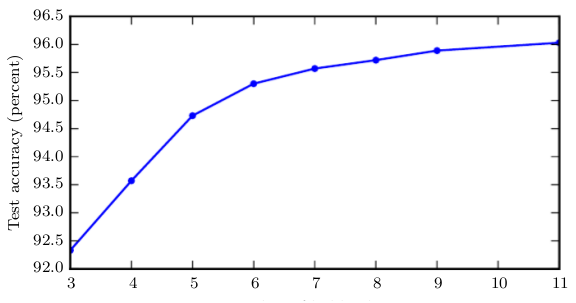
\includegraphics[width=0.475\linewidth]{figures/accuracy_depth.png}
      \hspace{0.2cm}
      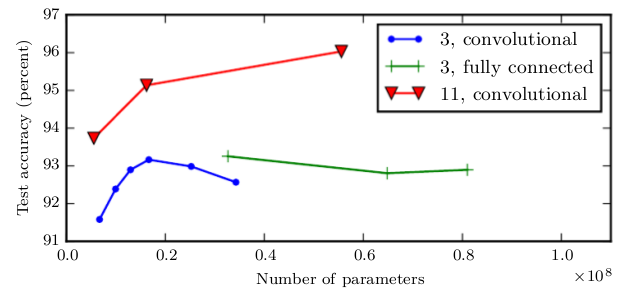
\includegraphics[width=0.475\linewidth]{figures/overfitting_depth.png}
   \end{figure}
\end{frame}

\begin{frame}
   {To sum up}
   \scriptsize
   \begin{itemize}
      \item
      A neural network is a function that takes a set of input $\left\lbrace x_i \right\rbrace$, and return a set of output $\left\lbrace y_i \right\rbrace$.
      \item
      This is done through a series of Linear transformations using linear weights $\boldsymbol{w}$, and non-linear function evaluations.
      \item
      Optimal weight parameters are found using an optimization/fitting algorithm, either using gradient or Hessian information.
      \item
      Network is evaluated by forward propagation.
      \item
      Derivatives of the linear weights are subsequently found by back propagation.
      \item
      Once optimal weight are found they can be stored and used for evaluating the network later.
   \end{itemize}
   
   \vspace{0.7cm}
   \begin{center}
      \normalsize
      \textbf{Take home message:} The Neural Network model is simply a non-linear function from a set of input variables $\left\lbrace x_i \right\rbrace$ to a set of output variables $\left\lbrace y_i \right\rbrace$ controlled by a vector $\boldsymbol{w}$ of adjustable parameters.
   \end{center}
\end{frame}

\begin{frame}
   {Flavors of Neural Networks}
   \vspace{-0.2cm}
   \begin{figure}
      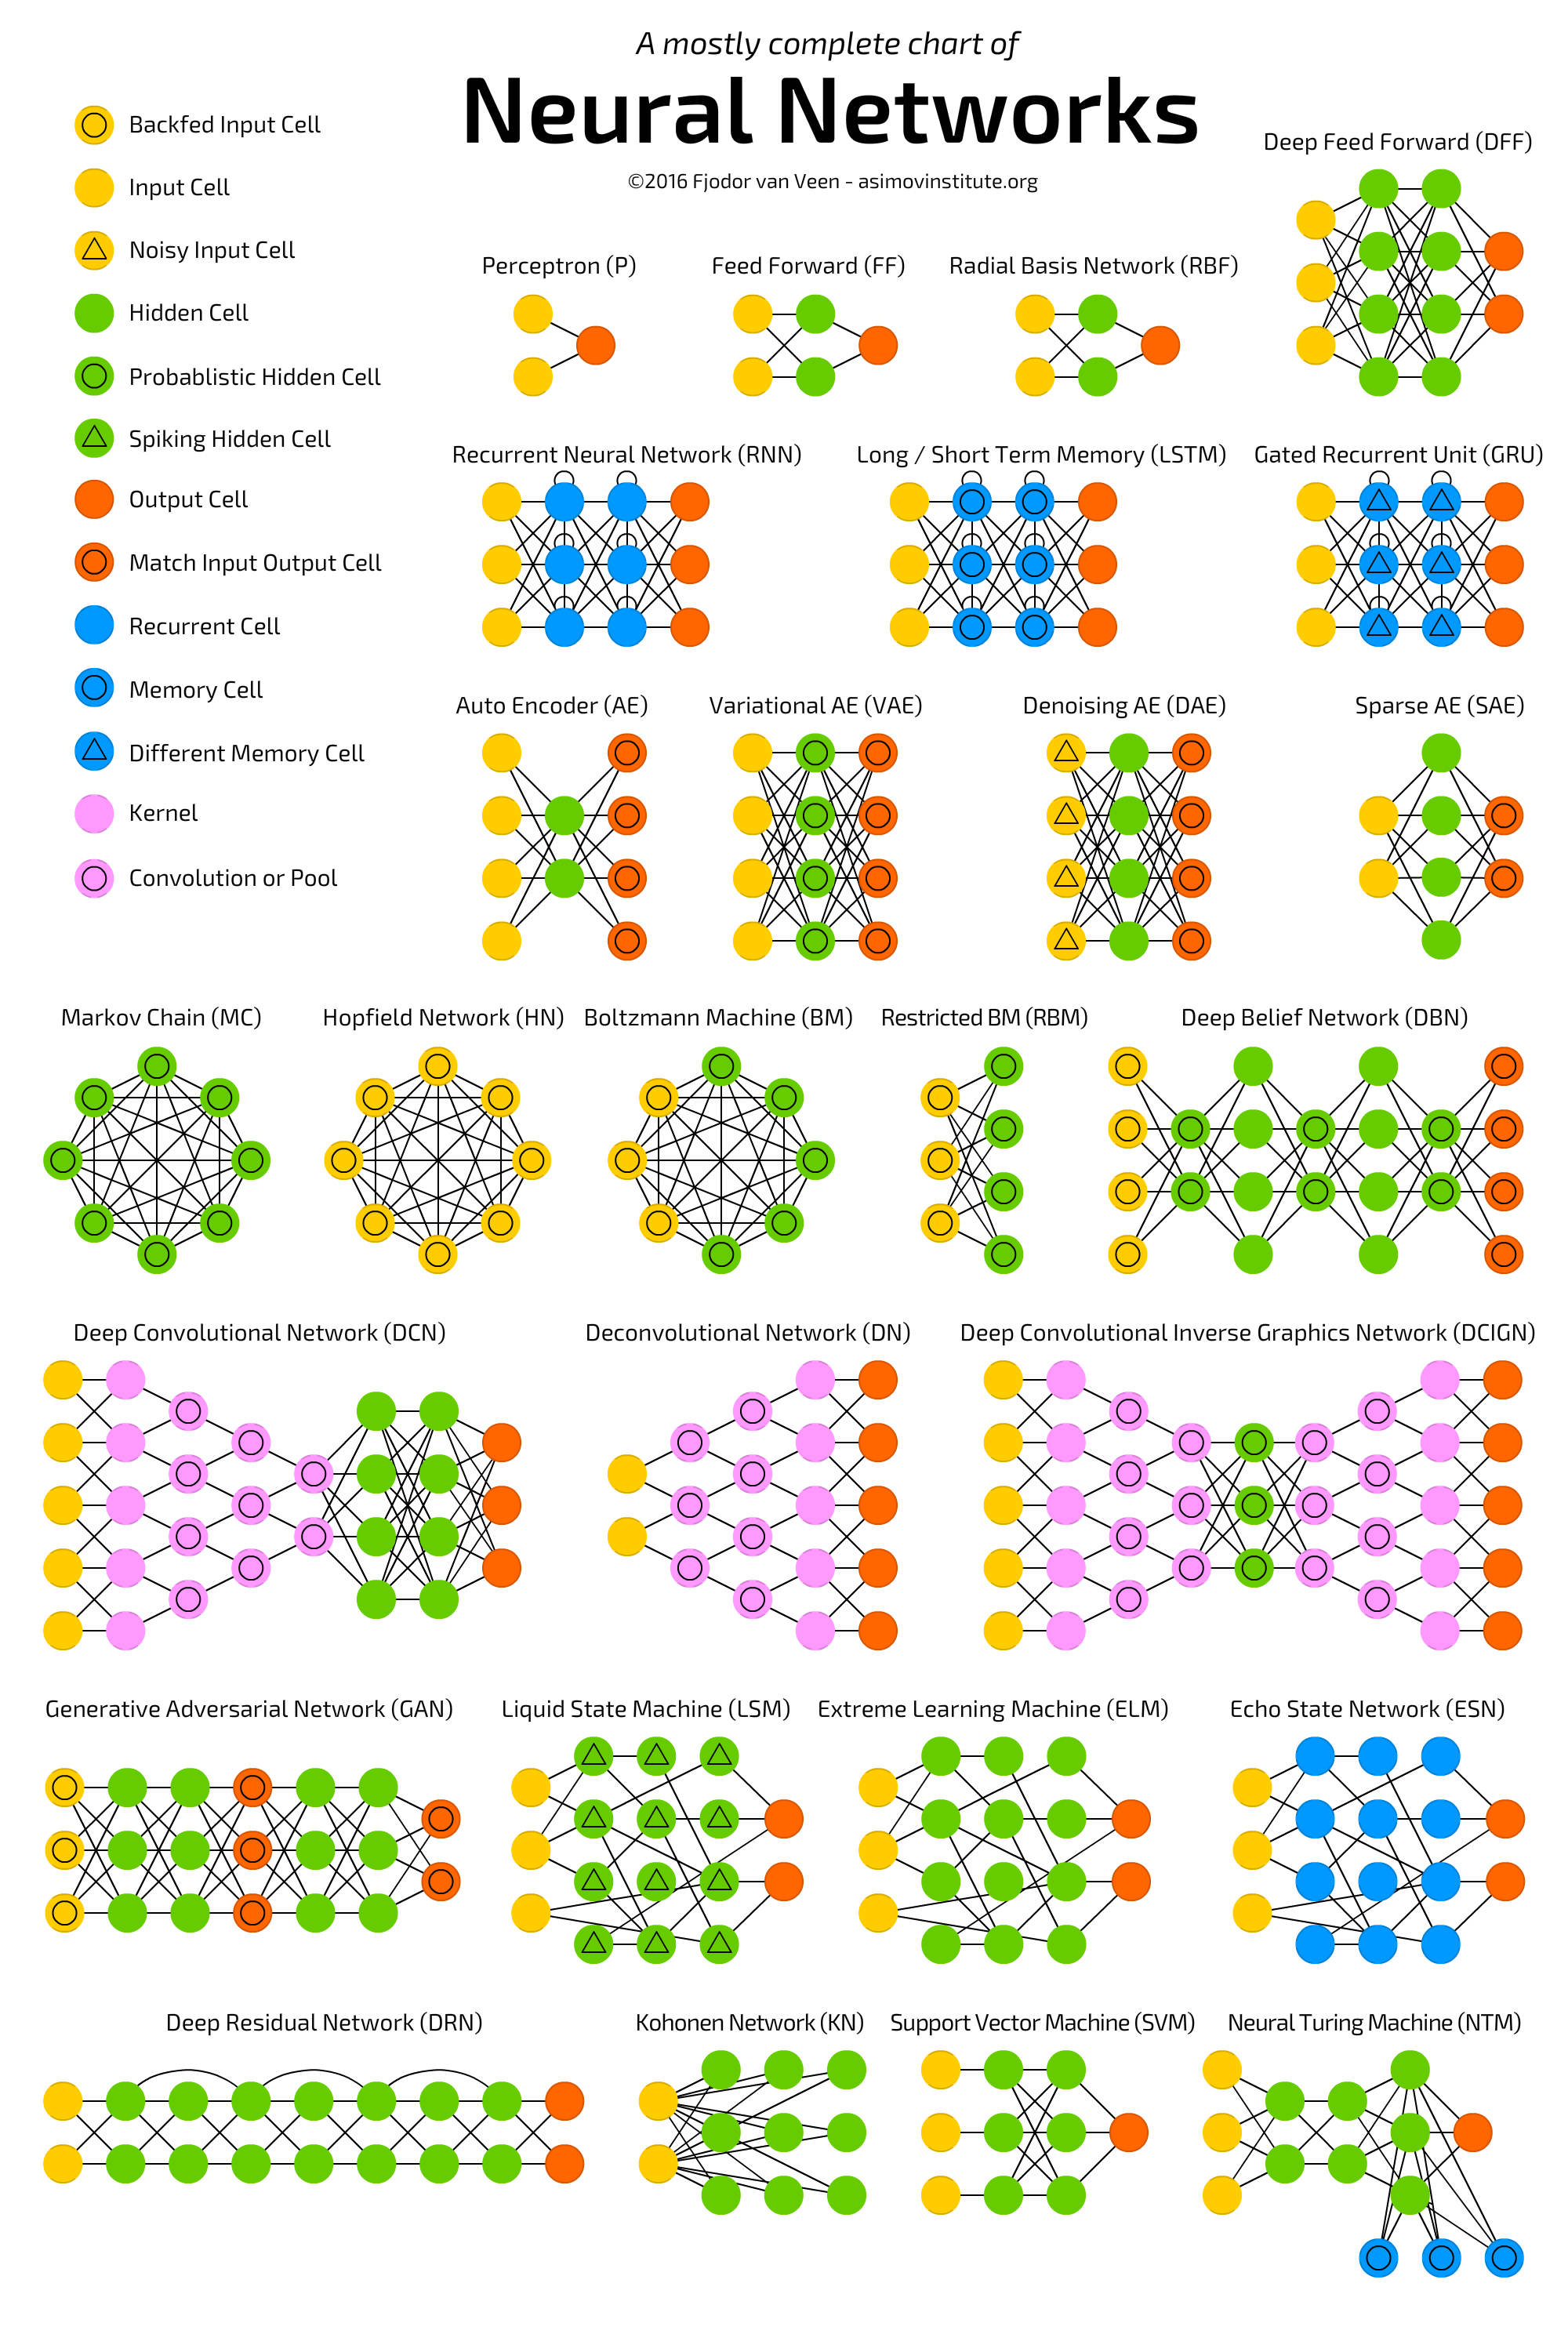
\includegraphics[scale=0.07]{figures/neuralnetworks.png}
   \end{figure}
\end{frame}

\begin{frame}
   {Resources}
   \scriptsize
   \vspace{-0.3cm}
   \begin{figure}
      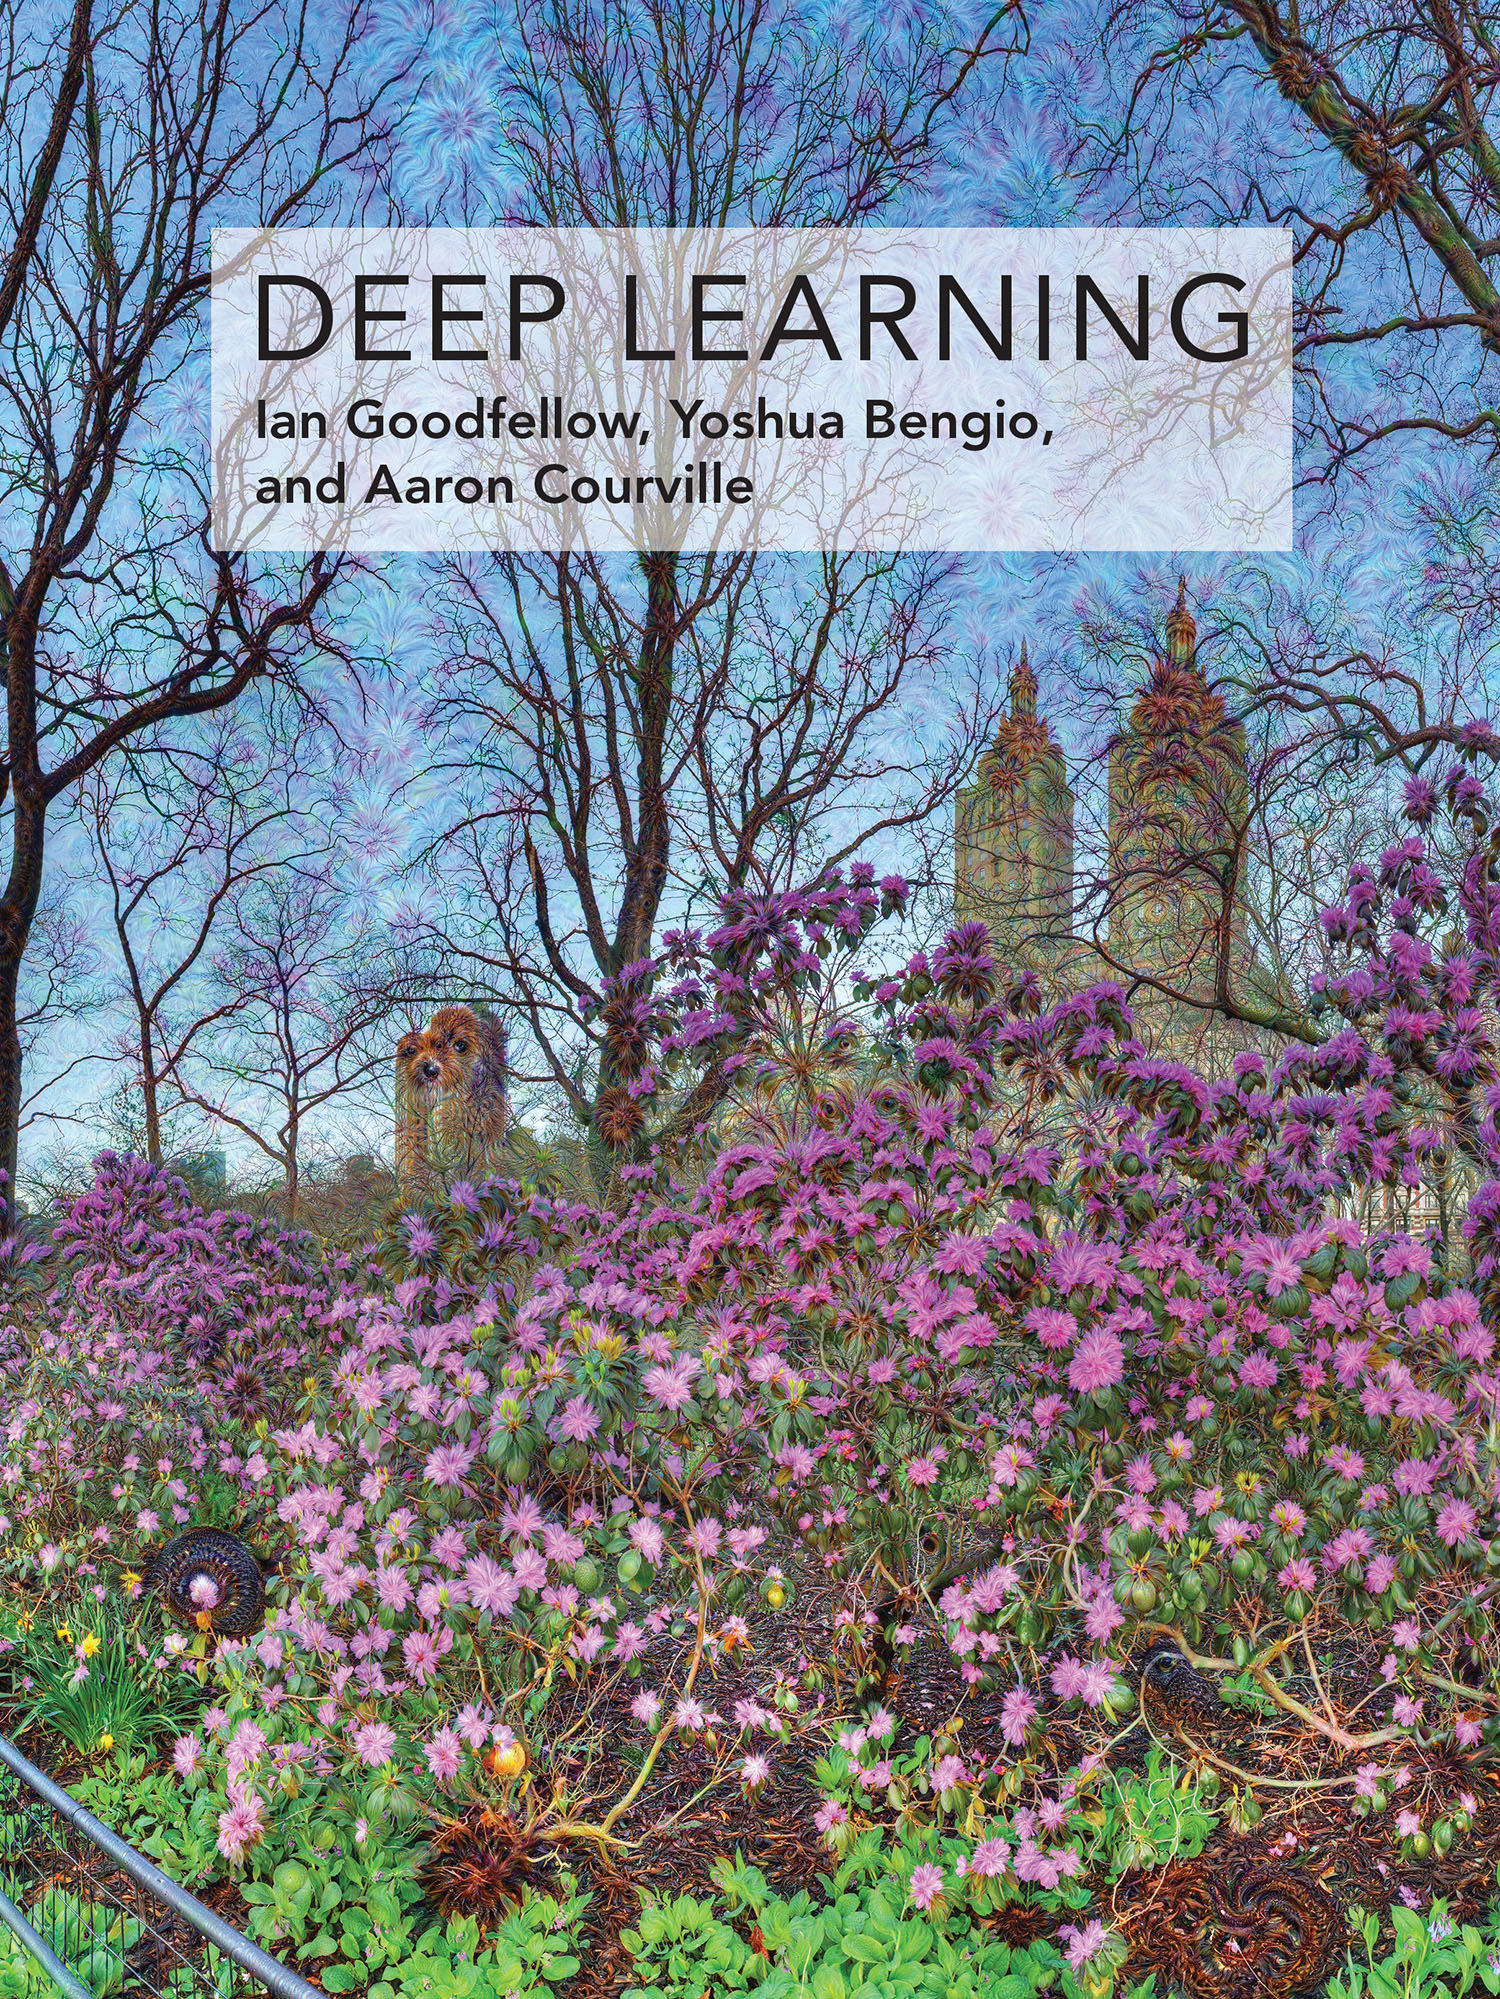
\includegraphics[scale=0.36]{figures/deep_learning_book.jpg}
   \end{figure}
   Available online: \url{http://www.deeplearningbook.org/} \newline \\
   And in pdf: \url{https://github.com/janishar/mit-deep-learning-book-pdf}
\end{frame}

\begin{frame}
   {And with that...}
   \begin{center}
   ... we are done for today!
   \end{center}
\end{frame}


\end{document}
